% REV00 Tue 20 Jul 2021 06:01:02 WIB
% START Tue 20 Jul 2021 06:01:02 WIB

\chapter{Pertama}

% 11
\begin{figure}[htbp]
% h: here, where the figure appears in the text (use can always just use [h] )
% t: top,  top of the current page.
% b: bottom of the current page.
% p: page, top of the next available float space (sometimes end up being the end of the document).
\centerline{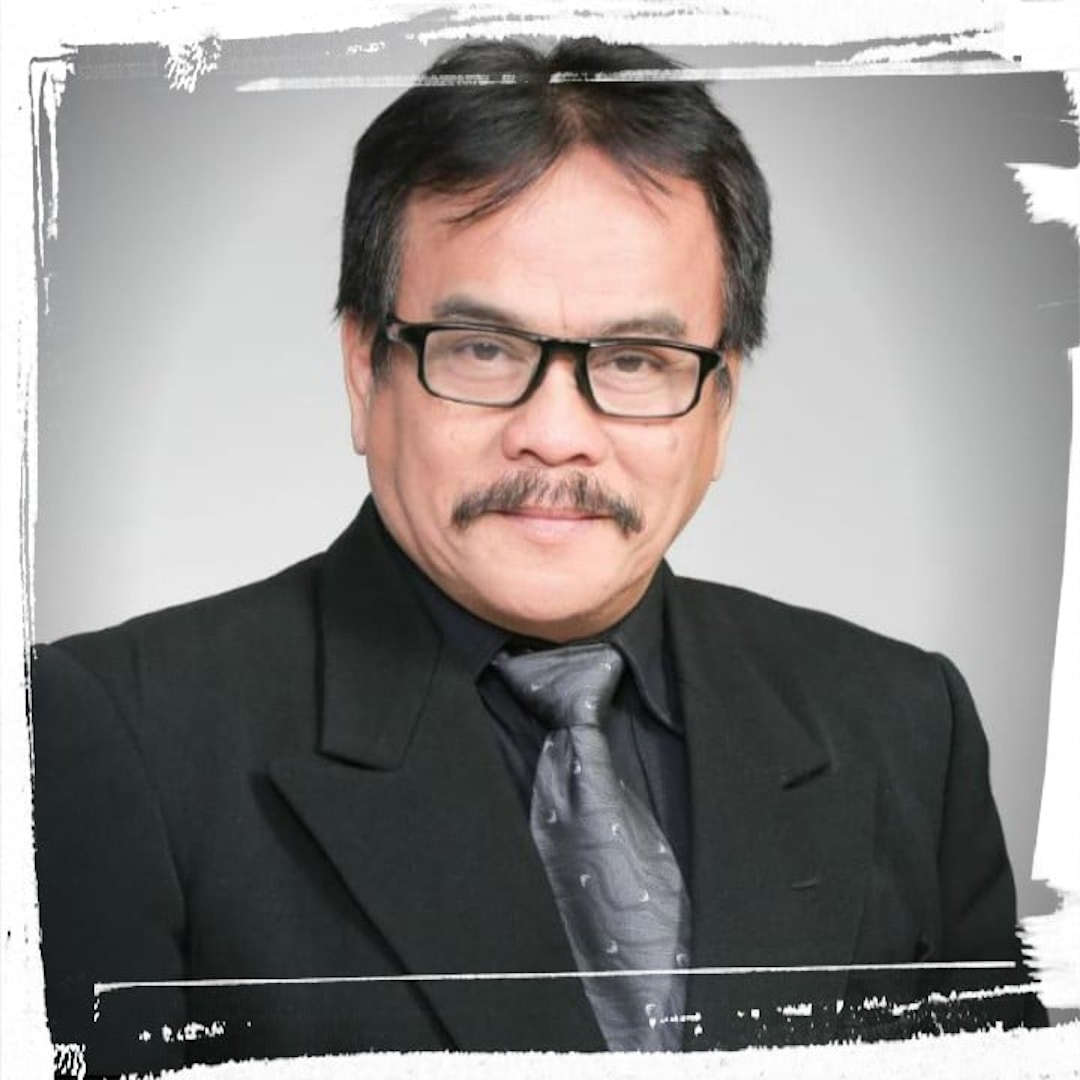
\includegraphics[scale=1.7]{01-01-01}}
\caption{Satiri on Facebook}
\label{01-01-01}
\end{figure}
%

\noindent
Kemarin dia kembali kepadaNya. Wabah buruk ini telah merengut jiwanya tanpa ampun. Seperti ditampar bolak-balik dalam mimpi buruk, kami amat sangat berduka. Bagiku, beliau adalah sahabat kehidupan. Friend for life. Dia adalah sosok yang seharusnya diberi gelar Pahlawan Betawi. Kisah hidupnya tidak kalah lebih sulitnya dari yang dialami Si Doel Anak Betawi, dan keberhasilan serta pengabdiannya jauh melampaui Si Doel Anak Modern.

Kami sama-sama masuk jurusan Fisika ITB, walupun pada tahun pertama kami tidak pada kelas yang sama, saya di T-03 dia di T-01. Jadi, tahun 1981 kami memulai perjalanan bersama menjadi sarjana fisika.

Dia mudah bergaul dengans semua orang, jenaka dan kadang cenderung jahil, walaupun tidak ada yang pernah sakit hati atas kejahilannya itu. Dan kami segera menjadi serumah, se-kontrakan, selama lebih dari tiga tahun. Kami sering saling bercerita dan saling mengunjungi keluarga masing-masing. Cerita ini saya coba susun sedapat mungkin sesuai dengan yang pernah diceritakannya kepada saya dan juga dari yang kami alami bersama. Bagaimanapun juga ini adalah cerita.

Dan inilah ceritanya.

Perjalanan fisika buat saya sangat berat, tetapi bagi Satiri ini hanya candaan semata. Ya, kita semua teman-temannya sadar belaka bahwa kecerdasannya melampaui semua teman sekelas. Ini agak berbeda dengan sobat kami BDU, yang lulus cum laude dengan nilai yang nyaris semuanya A. Satiri tidak cum laude, walau nilainya juga banyak A.

% 11
\begin{figure}[htbp]
% h: here, where the figure appears in the text (use can always just use [h] )
% t: top,  top of the current page.
% b: bottom of the current page.
% p: page, top of the next available float space (sometimes end up being the end of the document).
\centerline{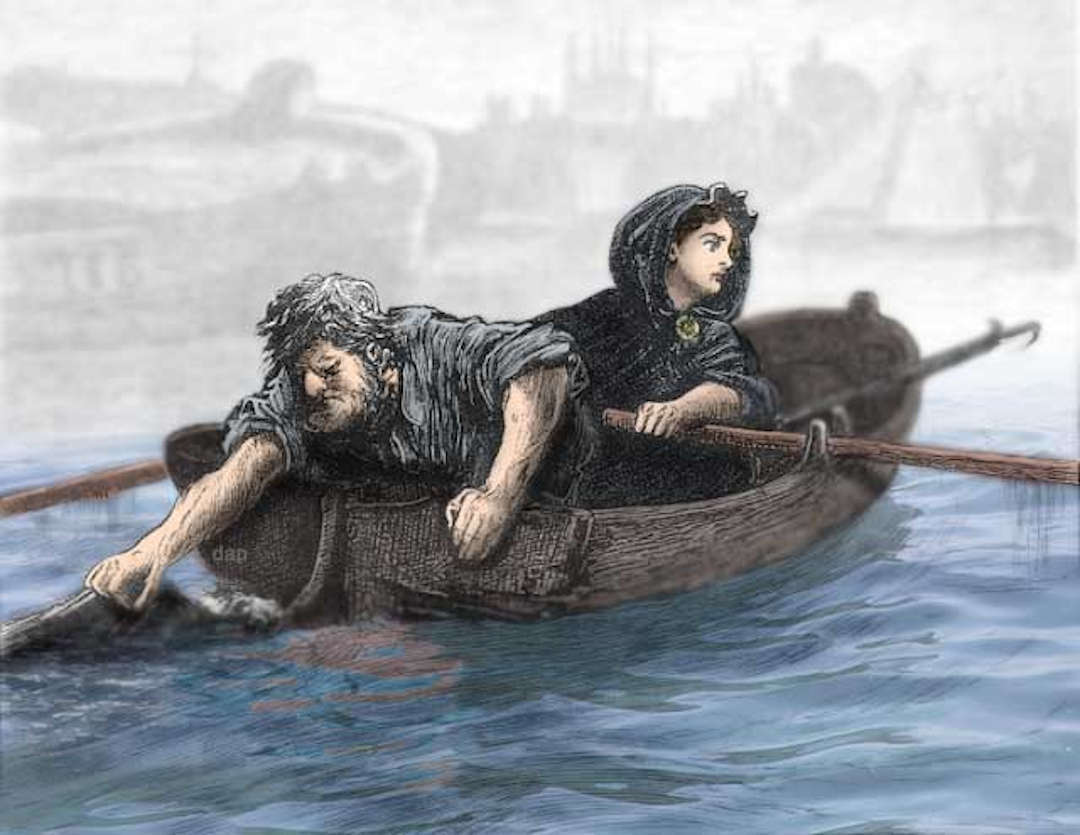
\includegraphics[scale=0.9]{01-01-02}}
\caption{Almarhum saat baru selesai wisuda (Aldi, Facebook)}
\label{01-01-02}
\end{figure}
%

BDU berasal dari keluarga yang sangat mampu. Kami menyebutnya mahasiswa tiga jurusan: Kamar kosnya yang mirip perpustakaan, ruang kelas, dan perpustakaan kampus. BDU orang yang baik hati, dan mau membantu teman-temannya. 'Kelas' (mutu) BDU jelas berbeda dengan 'kelas' saya, walaupun kami sekelas. Ketika kami memasuki kuliah di tahun ketiga, BDU sudah menjadi asisten dosen buat kami; dan dia bisa lulus dari ITB hanya dalam empat tahun, delapan semester, di tahun 1984. Padahal, saat itu program Sarjana ITB adalah 4,5 tahun dengan tiga tahun pertama adalah tingkat Sarjana Muda.

Meskipun demikian, menurutku kecerdasan Satiri jauh melampaui BDU. Kedua orang tua Satiri hanya sempat mengecap sedikit tahun di Sekolah Rakyat. Seingatku mereka tidak lancar membaca huruf latin, meskipun mereka sangat fasih membaca Al-Quran. Ayahnya pedagang kembang keliling, yang kadang mangkal di emperan Jalan Melawai, Blok M. Ibunya, seperti kebanyakan ibu-ibu di masa itu, berfokus untuk mengurus semua urusan rumah tangga.

Tahun 1982 saya mengunjungi rumah orang tua Satiri di sekitar Jalan Rawa Belong, Palmerah, Jakarta. Ya, dia orang Betawi asli yang lahir dan besar di kampung itu. Betawi adalah istilah untuk orang asli Jakarta. Betawi adalah pelafalan lokal dari "Batavia", nama yang diberikan Kolonial buat ibu kota Hindia Belanda (Indonesia).

Orang tua saya tinggal di bilangan Kampung Rawa, Simprug. Kami hanya terpisah beberapa kilometer saja. Rumahnya dapat dikatakan sangat sederhana, beralaskan tanah yang dikeraskan dan dengan dinding gedek (anyaman) bambu tipis diolesi kapur tebal. Di sanalah saya menemukan ibundanya dengan sinar mata yang terang dan suara yang lembut. Saya segera memahami bahwa inilah ibunda segala kebijasanaan dan kecerdasan! (Ibunda saya, nantilah saya ceritakan lain waktu)

Saat itu Satiri sudah punya istri dan satu orang anak! Ya, dia menikah, melalui drama yang tak kurang seru dari Drama Korea, waktu kami memasuki semester ke-2 di ITB. Nanti akan saya ceritakan juga drama tersebut jika memang memungkinkan. Sekarang, saya mau cerita dahulu bagaimana Satiri kecil berjalan tanpa alas kaki di semak belukar penuh bahaya, tanpa peta, untuk akhirnya tiba di kampus Ganesha.

Al Fatihah kami buat Bang Tiri, panggilan akbrabnya.
\\[10pt]
Sumber tulisan asli, \url{https://www.facebook.com/reno.alamsyah.94/posts/10226505323805448}.

